%%%%%%%%%%%%%%%%%%%%%%%%%%%%%%%%%%%%%%%%%%%%%%%%%%%%%%%%%%%
% --------------------------------------------------------
% Tau
% LaTeX Template
% Version 2.4.4 (28/02/2025)
%
% Author: 
% Guillermo Jimenez (memo.notess1@gmail.com)
% 
% License:
% Creative Commons CC BY 4.0
% --------------------------------------------------------
%%%%%%%%%%%%%%%%%%%%%%%%%%%%%%%%%%%%%%%%%%%%%%%%%%%%%%%%%%%

\documentclass[9pt,a4paper,twocolumn,twoside]{tau-class/tau}
\usepackage[english]{babel}
\usepackage{lipsum}
\usepackage[utf8]{inputenc}

\usepackage{pgfplots}
\usepackage{siunitx}
\usepgfplotslibrary{fillbetween}
\usetikzlibrary{patterns}  
\pgfplotsset{compat=1.18}

% Immagini come pdf
\usepackage{import}
\usepackage{xifthen}
\usepackage{pdfpages}
\usepackage{transparent}
\usepackage{hyperref}

\newcommand{\incfig}[1]{%
	\import{./img/}{#1.pdf_tex}
}

%\usepackage[siunitx]{circuitikz}

%% Spanish babel recomendation
% \usepackage[spanish,es-nodecimaldot,es-noindentfirst]{babel} 

%% Draft watermark
% \usepackage{draftwatermark}

%----------------------------------------------------------
% TITLE
%----------------------------------------------------------

\journalname{Torino, 28 maggio 2025}
\title{Esperienza di laboratorio: Costante di Planck}

%----------------------------------------------------------
% AUTHORS, AFFILIATIONS AND PROFESSOR
%----------------------------------------------------------

\author[b,c,3]{Mattia Benna, Federico Cesari, Matteo Herz}

%----------------------------------------------------------

%\affil[a]{Affiliation of author one}
%\affil[b]{Affiliation of author two}
%\affil[c]{Affiliation of author three}

\professor{Università di Torino - Corso di Laurea in Fisica}

%----------------------------------------------------------
% FOOTER INFORMATION
%----------------------------------------------------------

\institution{Unito fisica}
\theday{28 maggio, 2025}
\course{Esperimentazioni 2}


%----------------------------------------------------------
% ABSTRACT AND KEYWORDS
%----------------------------------------------------------

\begin{abstract}
L'esperimento mira, per mezzo dell'effetto fotoelettrico, alla dimostrazione del modello proposto da Einstein sulla natura quantizzata della radiazione elettromagnetica. Più precisamente si è misurato il potenziale di arresto degli elettroni per sei diverse lunghezze d'onda emesse da sei LED differenti al fine di poter dare un'approssimazione della costante di Planck. Tramite l'utilizzo di strumentazione amatoriale è stato estrapolato un valore di \(h'\) compatibile con quello teorico \(h\) entro poco più di una volta la sua incertezza.
\end{abstract}

%----------------------------------------------------------

%\keywords{filtro passa-banda, circuito RLC, guadagno}

%----------------------------------------------------------

\begin{document}
		
    \maketitle 
    \thispagestyle{firststyle} 
    \tauabstract
    % \tableofcontents
    % \linenumbers 
    
%----------------------------------------------------------
\vspace{-0.8cm}
\section{Introduzione}
Quest'esperimento si basa sulle intuizioni geniali che Planck ed Einstein ebbero agli inizi del '900 e che diedero il via alla teoria della meccanica quantistica. La costante di Planck è inoltre una delle principali costanti presenti in tutta la fisica dei sistemi subnucleari e non solo, ed è incredibile pensare che con un esperimento relativamente semplice si possa ottenere una costante così importante e all'apparenza completamente al di fuori della nostra vita quotidiana.


\section{Nozioni teoriche}
Per ricavare l'energia trasportata dai fotoni emessi dai led sfruttiamo l'effetto fotoelettrico: secondo la teoria poposta da Einstein gli elettroni che vengono colpiti dai fotoni, aventi sufficiente energia, vengono estratti dal metallo acquistando un'energia cinetica:
\[
    E_k= h \nu - W_e
\]
dove \(h = 6.63 \times 10^{-34} \text{Js}\) è la costante di Planck, \(\nu\) è la frequenza della radiazione incidente  e \(W_e\) è il lavoro di estrazione, valore caratteristico di ogni metallo, corrispondente all'energia necessaria per liberare un elettrone da un suo atomo.

Per ricavare sperimentalmente l'energia cinetica degli elettroni si fornisce una tensione di contro-campo tra anodo e catodo, questa si oppone al moto degli elettroni, fino ad arrestarli raggiunto un valore di tensione \(V_0\). In questa condizione vale l'equazione:
\[
    E_k  = e V_0  = h\nu - W_e
\]

\section{Apparato e procedura sperimentale}

L'apparato sperimentale è composto dai seguenti elementi:
\begin{itemize}
    \item Contenitore schermato: involucro per tenere nella completa oscurità la strumentazione fotosensibile,
    \item pile da 5V per alimentare il contro-campo,
    \item potenziometro per regolare l'intensità del contro-campo,
    \item microamperometro per misurare la corrente generata dagli elettroni,
    \item generatore di corrente continua per alimentare il led.
    \item 6 led con diverse lunghezze d'onda:
\end{itemize}

 \begin{table}[H]
    \centering
    \begin{tabular}{@{}lcc@{}}
        \toprule
        \textit{led} & \(\lambda\) (nm) & \(\sigma_\lambda\) (nm) \\
        \midrule
        \textit{1} & 430 & 1 \\
        \textit{2} & 470 & 1 \\
        \textit{3} & 558 & 4 \\ 
        \bottomrule  
    \end{tabular}
    \hspace{1cm} % Adjust spacing between tables as needed
    \begin{tabular}{@{}lcc@{}}
        \toprule
        \textit{led} & \(\lambda\) (nm) & \(\sigma_\lambda\) (nm) \\
        \midrule
        \textit{4} & 595 & 5 \\
        \textit{5} & 605 & 1 \\
        \textit{6} & 644 & 2 \\ 
        \bottomrule  
    \end{tabular}
    \caption{Led utilizzati con relativa lunghezza d'onda.}
\end{table}
    
\begin{figure}[H]
    \centering
    \incfig{photo_1}
    \caption{Apparato sperimentale}
\end{figure}

Prima di cominciare la misura sono necessari alcuni accorgimenti: scelto e posizionato il led nel suo apposito scomparto è necessario chiudere attentamente il contenitore per fare in modo che la luce dell'ambiente non influisca sulla misura. Abbiamo poi misurato la "corrente di fondo" registrata dal microamperometro a led spento; a tutte le misure della corrente verrà sottratto il valore della corrente di fondo. 

Posizionato il led sul supporto si aumenta, tramite il potenziometro, la tensione \(V\) di controcampo a intervalli regolari e si registra per ogni valore di \(V\) letto dal multimetro la corrente \(I\) registrata dal microamperometro.  All'aumentare di \(V\) la corrente diminuisce fino, idealmente, ad appiattirsi intorno allo zero, o almeno così ci si aspetta che accada se la strumentazione è perfettamente tarata. Le misure vanno ripetute identicamente per tutti e sei i led a disposizione. 

Riportiamo un grafico di esempio:
\begin{figure}[H]
\centering
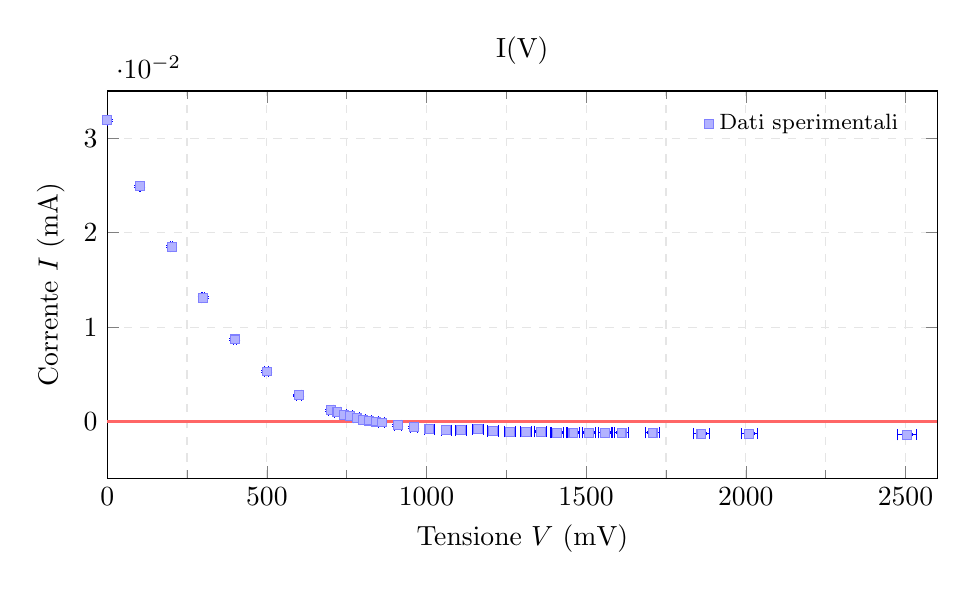
\begin{tikzpicture}
		\begin{axis}[
			title={I(V)},
			xlabel={Tensione \(V\) (mV)},
			ylabel={Corrente \(I\) (mA)},
			grid=both,
			grid style={dashed, gray!20},
			height=6.5cm,
                width=\linewidth,
			legend pos=north east,
			xmin=0,
			xmax=2600,
			ymin=-0.006,
			ymax=0.035,
			xtick={0,500,1000,1500,2000,2500}, % Tick uniformemente spaziati
			xticklabels={0,500,1000,1500,2000,2500}, % Etichette ordinate
			minor xtick={250,750,1250,1750,2250}, % Tick minori per migliore leggibilità
			error bars/x dir=both,
			error bars/y dir=both,
			error bars/x explicit,
			error bars/y explicit,
                legend style={
                    draw=none,
                    fill=none,
                    text opacity=1,
                    font=\footnotesize,
                    cells={anchor=east}
                }
			]
			
			% Dati con errori
			\addplot+ [
			only marks,
			mark=square*,
			mark options={solid, fill=blue!30, draw=blue!50, scale=0.8},
			] table [x error=x_v_err, y error=y_i_err] {
				x       y       x_v_err   y_i_err
				0.50    0.0319  0.5       0.0001
				102.5   0.0249  2         0.0001
				201.9   0.0185  3         0.0001
				300.9   0.0131  4         0.0001
				400.1   0.0087  5         0.0001
				500.0   0.0053  6         0.0001
				600.5   0.0028  7         0.0001
				700.4   0.0012  8         0.0001
				721.0   0.0010  8         0.0001
				740.5   0.0007  8         0.0001
				759.9   0.0006  8         0.0001
				781.1   0.0004  8         0.0001
				801.0   0.0002  9         0.0001
				819.7   0.0001  9         0.0001
				841.0   0.0000  9         0.0001
				859.9   -0.0001 9         0.0001
				910.4   -0.0004 10        0.0001
				960.6   -0.0006 10        0.0001
				1009.0  -0.0008 15        0.0001
				1062.0  -0.0009 16        0.0001
				1108.0  -0.0009 16        0.0001
				1162.0  -0.0008 17        0.0001
				1209.0  -0.0010 17        0.0001
				1261.0  -0.0011 18        0.0001
				1311.0  -0.0011 18        0.0001
				1358.0  -0.0011 19        0.0001
				1409.0  -0.0012 19        0.0001
				1460.0  -0.0012 20        0.0001
				1509.0  -0.0012 20        0.0001
				1560.0  -0.0012 21        0.0001
				1611.0  -0.0012 21        0.0001
				1708.0  -0.0012 22        0.0001
				1861.0  -0.0013 24        0.0001
				2011.0  -0.0013 25        0.0001
				2505.0  -0.0014 30        0.0001
			};
			\addplot[
			red!60, 
			thick, 
			domain=0:2600, 
			samples=200
			] {
				0
			};
			\legend{Dati sperimentali}
		\end{axis}
	\end{tikzpicture}
    \caption{Andamento della corrente in funzione della tensione di controcampo per il LED con \(\lambda = 430\) nm.}
\end{figure}


\section{Analisi dati e discussione}
Si è deciso di associare come errore sulle misure di corrente la prima cifra oscillante, mentre per le misure di tensione abbiamo seguito le indicazioni date dal costruttore del voltmetro.
Da una prima analisi dei set di dati è chiaro che determinare la corrente di plateau non risulta conveniente: l'andamento della corrente infatti non si appiattisce sullo zero ma tende verso valori sempre più negativi. Questo probabilmente è dovuto a fotoelettroni emessi dall'anodo per luce diffusa nella camera ed essi vengono spinti verso il catodo, dalla tensione di contro campo, generando una corrente inversa %\footnote{Proprio perché si suppone che questi elettroni siano emessi dall'anodo crediamo che tale corrente negativa non sia dipendente dalla tensione di controcampo applicata.}.

Abbiamo dunque optato per un altro metodo di analisi: abbiamo scelto come tensione di arresto la tensione associata al valore di corrente più vicino allo zero. Tutti i valori di corrente scelti sono in un intorno di zero entro l'errore associato. Per ogni led, di cui erano note le lunghezze d'onda si è ricavata la frequenza \(\nu = c/\lambda\) così da ottenere la coppia di valori \(V_0,\nu\) per ogni LED. 

\begin{table}[H]
            \centering
            \begin{tabular}{lcccc}
                \toprule
                 \textit{led}&\(\Delta V_0\) (mV) & \(\sigma_{\Delta V_0}\) (mV) & \(\Delta\nu\) (THz) &  \(\sigma_{\Delta \nu}\) (THz)\\
                \midrule
                \textit{1-2} &230 & 16 & 59.3& 2.1 \\
                \textit{2-3} &400 & 9  & 101.0 & 4.1 \\
                \textit{3-4} &50 & 5  & 8.3&  4.3 \\
                \textit{4-5} &10  & 5  & 33.4 & 5.7 \\
                \textit{5-6} &30  & 4  & 30.0 & 1.7 \\
                \bottomrule  
            \end{tabular}
            \caption{Differenze dei potenziali di arresto e delle frequenze utilizzati per la retta di best-fit.}
            %\tabletext{Note: se c'è qualcosa da far notare: quì!}
\end{table}
Gli errori associati alla differenza del potenziale d'arresto \(\sigma_{\Delta V_0}\) sono stati ricavati sommando le incertezze associate a ciascun potenziale. Poiché l'andamento del potenziale è influenzato anche dalla corrente, influenza di cui non abbiamo potuto tener conto, associare l'errore in quadratura avrebbe portato a una probabile sottostima dell'errore.

Per ricavare il valore della costante di Planck \(h'\) abbiamo tracciato la retta di best fit con i dati ottenuti:
\[
\Delta V_0 = \frac{h'}{e}\Delta\nu
\]
 Così da poter estrapolare \(h'\) dal suo coefficiente angolare (sapendo che \(e = 1.602\times 10^{-19}\) C è la carica dell'elettrone). 

Da una prima analisi due punti risultano essere non compatibili con l'andamento lineare che ci aspettiamo. Infatti le prese dati dei led 5 e 6 sono visibilmente peggiori delle altre: non seguono l'andamento atteso specialmente nella zona di plateau. Questo ci porta a pensare a problemi esterni legati all'apparato o ai led in questione. Escludendo i dati dei LED 5 e 6 otteniamo il seguente fit:

\begin{table}[H]
            \centering
            \begin{tabular}{lcccc}
                \toprule
                 \textit{led}&\(\Delta V_0\) (mV) & \(\delta_{\Delta V_0}\) (mV) & \(\Delta\nu\) (THz) &  \(\delta_{\Delta \nu}\) (THz)\\
                \midrule
                \textit{1-2} &230 & 16 & 59.3& 2.1 \\
                \textit{2-3} &400 & 9  & 101.0 & 4.1 \\
                \textit{3-4} &50 & 5  & 8.3&  4.3 \\
                \bottomrule  
            \end{tabular}
            \caption{Differenze dei potenziali di arresto e delle frequenze utilizzati per la retta di best-fit escluse le prese dati peggiori corrispondenti ai LED 5 e 6.}
            %\tabletext{Note: se c'è qualcosa da far notare: quì!}
\end{table}

\begin{figure}[H]
\centering
    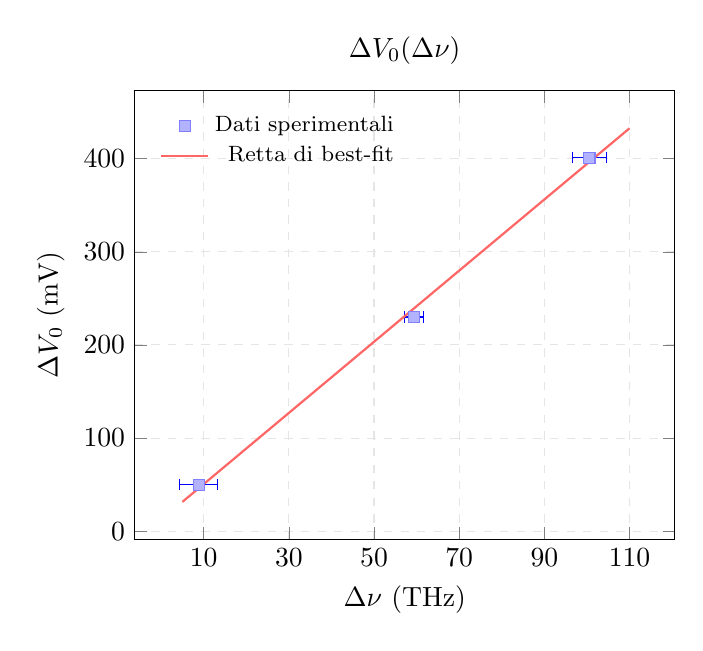
\begin{tikzpicture}
    \begin{axis}[
        title={\(\Delta V_0 (\Delta \nu)\)},
        xlabel={\(\Delta \nu\) (THz)},
        ylabel={\(\Delta V_0\) (mV)},
        xtick={10,30,50,70,90,110},
        xticklabels={10,30,50,70,90,110},
        scaled x ticks=false,  
        x tick label style={/pgf/number format/.cd, fixed},
        grid=both,
        grid style={dashed, gray!20},
        legend pos=north west,
        legend style={
            draw=none,
            fill=none,
            text opacity=1,
            font=\footnotesize,
            cells={anchor=east}
        }
        ]
        
        % Dati principali (quadrati blu)
        \addplot+ [
        only marks,
        mark=square*,
        mark options={solid, fill=blue!30, draw=blue!50, scale=1},
        error bars/.cd,
        x dir=both,
        x explicit,
        y dir=both,
        y explicit
        ] table [x error=xerror] {
            x        y    xerror   error
            59.34    230  2.2114   16
            100.59   401  4.083    9
            8.8328   50   4.4313   5
        };
        \addlegendentry{Dati sperimentali}
        
        \addplot[
        red!60, 
        thick, 
        domain=5:110, 
        samples=200
        ] {
            3.82*x + 12.37  % Nuova retta di best-fit (valori approssimati)
        };
        \addlegendentry{Retta di best-fit}
        
\end{axis}
\end{tikzpicture}
\caption{Fit lienare: \(\Delta V_0 = h'/e \Delta \nu\) con i valori riportati in \textbf{Table 3}.}
\end{figure}
Da cui si ottiene il coefficiente angolare della retta
\[
\frac{h'}{e} = 3.82 \pm 0.27 \: \frac{\text{Js}}{\text{C}}
\]
e conseguentemente il valore di \(h\)
\[
\boxed{h' = 6.12 \pm 0.45 \, \times 10^{-34} \text{Js}}
\]
valore compatibile con quello teorico entro circa una volta l'incertezza (\( \approx 1.2\) volte).

\section{Conclusioni}
L'esperimento ha permesso di studiare l'effetto fotoelettrico e di stimare il valore della costante di Planck attraverso la misura della corrente elettrica generata dall'irraggiamento di un catodo metallico con LED a diverse lunghezze d'onda.

Nonostante due dei sei LED utilizzati non abbiano prodotto set di dati coerenti con il modello teorico, tramite le misure ottenute dai primi quattro siamo stati in grado di ricavare un'approssimazione della costante di Planck sorprendentemente accurata: compatibile entro \(\approx 1.2\) volte la sua incertezza \(\delta_{h'}\).


\end{document}